\section{A Long List of Lemmas}
From this point forward in the section we assume that \(\DConf_n(\Gamma)\) is an \(m\)-manifold without boundary
and \(M\) is an \((m-1)\)-matching in \(\Gamma\).

\subsection{Minimum Graph Size and Key Lemma}

\begin{lem}
\label{lem:graph-size}
    \(\Gamma\) has at least \(m + n\) vertices and \(n \ge m\).
\end{lem}

\begin{proof}
    If \(\Gamma\) has less than \(n\) vertices, then \(\DConf_n(\Gamma)\) is empty;
    so, suppose \(\Gamma\) has at least \(n\) vertices.
    If \(\Gamma\) has less than \(n + m\) vertices, then
    for any configuration of \(n\) particles on \(\Gamma\)
    at most \(m-1\) particles can simultaneously move.
    Since exactly \(m\) particles need to be able to simultaneously move for an \(m\)-cube 
    to exist in \(\DConf_n(\Gamma)\), no configuration in \(\DConf_n(\Gamma)\)
    can have a neighborhood homeomorphic to an open set in \(\mathbb{R}^m\).

    Similarly, if \(n < m\), then there are not enough particles that can simultaneously move
    for an \(m\)-cube to exist in \(\DConf_n(\Gamma)\). So, \(n \ge m\). 
\end{proof}

This next lemma is the key to all following proofs.
The idea is that if we have an \((m-1)\)-cube in the configuration space,
then there needs to be exactly two \(m\)-cubes that border it for the points
in that \((m-1)\)-cube to look locally like \(\mathbb{R}^m\).

\begin{lem}
    \label{lem:special-edges}
    For any collection \(\mathcal{V}\) of \(n - (m - 1)\) vertices in \(\Gamma - V(M)\), there exists exactly \textbf{two}
    edges \(e_1\) and \(e_2\) in \(\Gamma - V(M)\) that are incident to vertices in \(\mathcal{V}\)
    and vertices not in \(\mathcal{V}\).

    Furthermore, these edges \(e_1\) and \(e_2\) satisfy all of the following conditions.
    \begin{enumerate}[label=(\roman*)]
    \item \(e_1\) and \(e_2\) are both incident to one vertex in \(\mathcal{V}\)
    \item \(e_1\) and \(e_2\) are both incident to one vertex not in \(\mathcal{V}\)
    \item \(e_1\) and \(e_2\) share exactly one common vertex.
    \end{enumerate}

    Equivalently, exactly one of the following hold in Figure \ref{fig:lem:special-edges}
    \begin{figure}[h!]
        \centering
        \begin{enumerate*}[label=(\arabic*)]
            \item \label{fig:lem:manifolds_1_1}
            \begin{minipage}{.3\textwidth}
                \centering
                \(v_1 \in \mathcal{V}\) \textit{and} \(w_1, w_2 \not \in \mathcal{V}\) \\
                \vspace{1em}
                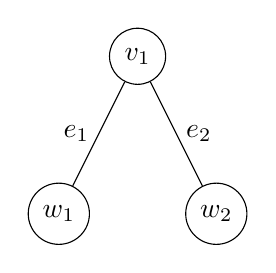
\begin{tikzpicture}
                    \node (v1) at (3, 2) [circle, draw] {\(v_1\)};
                    \node (w1) at (2, 0) [circle, draw] {\(w_1\)};
                    \node (w2) at (4, 0) [circle, draw] {\(w_2\)};

                    \draw (v1) -- (w1) node[midway, left] {\(e_1\)};
                    \draw (v1) -- (w2) node[midway, right] {\(e_2\)};
                \end{tikzpicture} 
            \end{minipage}

            \hspace{3em}

            \item \label{fig:lem:manifolds_1_2}
            \begin{minipage}{.3\textwidth}
                \centering
                \(v_1, v_2 \in \mathcal{V}\) \textit{and} \(w_1 \not \in \mathcal{V}\) \\
                \vspace{1em}
                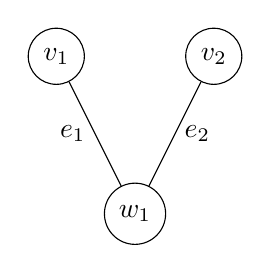
\begin{tikzpicture}
                    \node (v1) at (2, 2) [circle, draw] {\(v_1\)};
                    \node (v2) at (4, 2) [circle, draw] {\(v_2\)};
                    \node (w1) at (3, 0) [circle, draw] {\(w_1\)};

                    \draw (v1) -- (w1) node[midway, left] {\(e_1\)};
                    \draw (v2) -- (w1) node[midway, right] {\(e_2\)};
                \end{tikzpicture}
            \end{minipage}
        \end{enumerate*}
        \caption{Lemma \ref{lem:special-edges} possibilities.}
        \label{fig:lem:special-edges}
    \end{figure}
\end{lem}

\begin{proof}
    Let \(\mathcal{V}\) be a collection of \(n - (m - 1)\) vertices in \(\Gamma - V(M)\)
    and \(p\) be the configuration of \(n\) particles placed on \(\Gamma\) such that
    \(n - (m - 1)\) particles are placed at each vertex in \(\mathcal{V}\)
    and \(m - 1\) particles on each edge in \(M\).
    
    As the particles move move along the edges in \(M\), an \((m-1)\)-cube containing \(p\)
    is spanned in \(\DConf_n(\Gamma)\).
    Since the configuration space is an \(m\)-manifold without boundary, 
    this \((m-1)\)-cube must border exactly two distinct \(m\)-cubes.
    For this \((m-1)\)-cube to border two \(m\)-cubes,
    there needs to exist \textbf{two} additional mutually exclusive particle movements.
    Let \(v_1, v_2 \in \mathcal{V}\) and \(w_1, w_2 \not \in \mathcal{V}\) be the vertices corresponding
    to the origins and destinations of these additional particle movements.
    If \(v_1 \neq v_2\) and \(w_1 \neq w_2\), then two particles would be able to move simultaneously
    resulting in an \((m+1)\)-cube being spanned in \(\DConf_n(\Gamma)\) contradicting 
    that it is an \(m\)-manifold.
\end{proof}

\subsection{\(m = 1\) or No Cycles}

\begin{lem}
    \label{lem:manifold-max-degree}
    Every vertex in \(\Gamma - V(M)\) has degree at most \(3\).
\end{lem}

\begin{proof}
    Suppose \(\Gamma - V(M)\) has a vertex \(v\) with degree greater than \(3\).
    We proceed by cases on \(n\).

    \textbf{Case 1:} \(n \le m - 1 + \deg(v)\)
    In the context of Lemma \ref{lem:special-edges},
    construct \(\mathcal{V}\) so that all \(n - (m - 1) = n - m + 1\)
    vertices are on the vertices adjacent to \(v\).
    Then, there are too many edges with one endpoint in \(\mathcal{V}\)
    and other outside of \(\mathcal{V}\) for Lemma \ref{lem:special-edges} to hold.

    \textbf{Case 2:} \(n > m - 1 + \deg(v)\)
    Lemma \ref{lem:graph-size} guarantees that \(\Gamma - V(M)\) has at least
    \(n + m - 2(m - 1) = n - m + 2\) vertices.
    So, \(\abs{V(\Gamma - V(M))} > \deg(v) + 1\).
    More importantly, it's clear now that we can now construct a \(\mathcal{V}\)
    so that it contains \(v\) and every vertex adjacent to \(v\).
    By Lemma \ref{lem:special-edges}, there is at least one vertex \(w \not \in \mathcal{V}\).
    Let \(\mathcal{V}' = \left(\mathcal{V}\setminus\{v\}\right)\cup\{w\}\) i.e. 
    swap out \(v\) for \(w\) in \(\mathcal{V}\).
    Then, again there are now too many edges with one endpoint in \(\mathcal{V}'\)
    and another outside of \(\mathcal{V}'\) to for Lemma \ref{lem:special-edges} to hold.
\end{proof}

\begin{lem}
    \label{lem:manifold-is-claw}
    If \(\Gamma - V(M)\) contains a degree \(3\) vertex,
    then \(\Gamma - V(M) \cong K_{1,3}\) and \(n = m + 1\).
\end{lem}

\begin{proof}
    Suppose \(\Gamma - V(M)\) contains a degree \(3\) vertex \(v\).
    First we show that \(n\) must be equal to \(m + 1\) by considering two cases.

    \textbf{Case 1:} \(n > m + 1\)
    % TODO Clean up
    Fill up the \(Y\)-graph.
    There must be at least one free vertex.
    Put a particle there instead of at \(v\)
    Book.

    \textbf{Case 2:} \(n < m + 1\)
    In this case \(n\) must equal \(m\) by Lemma \ref{lem:graph-size}.
    Let \(\mathcal{V}\) consist of just the vertex \(v\).
    Then, there are too many edges with one endpoint in \(\mathcal{V}\)
    and another outside of \(\mathcal{V}\) to for Lemma \ref{lem:special-edges} to hold.
    Namely, the three edges incident to \(v\).

    Now we show that there cannot be any other vertices in \(\Gamma - V(M)\) besides \(v\) and its neighbors.
    Suppose there was a vertex \(w \neq v\) in \(\Gamma - V(M)\) that is not adjacent to \(v\).
    Let \(\mathcal{V} = \{v, w\}\).
    Then, again there are too many edges with one endpoint in \(\mathcal{V}\)
    and another outside of \(\mathcal{V}\) to for Lemma \ref{lem:special-edges} to hold.
    Namely, the three edges incident to \(v\).

    Finally, we show that there cannot be any edges in \(\Gamma - V(M)\)
    besides the three edges incident to \(v\).

    Suppose there was another edge \(e\) in \(\Gamma - V(M)\) not incident to \(v\) and
    let \(a\) and \(b\) be the vertices incident to \(e\) and \(c\) be the other vertex adjacent to \(v\)
    (see Figure \ref{fig:lem:manifold-is-claw-1}).

    \begin{figure}
        \centering
        \begin{tikzpicture}
            \node (v) at (0,0) [circle, draw] {\(v\)};
            \node (a) at (-2,-2) [circle, draw] {\(a\)};
            \node (b) at (2,-2) [circle, draw] {\(b\)};
            \node (c) at (0,2) [circle, draw] {\(c\)};

            \draw (v) -- (a);
            \draw (v) -- (b);
            \draw (v) -- (c);
            \draw (a) -- (b) node[midway, below] {\(e\)};
        \end{tikzpicture}
        \caption{\(\Gamma - V(M)\) with an extra edge \(e\)}
        \label{fig:lem:manifold-is-claw-1}
    \end{figure}

    Let \(\mathcal{V} = \{a, c\}\).
    Then, again there are too many edges with one endpoint in \(\mathcal{V}\) and another outside of \(\mathcal{V}\).
    Namely, \(cv\), \(av\), and \(bv\).

    Therefore \(\Gamma - V(M)\) must consist solely of \(v\), its neighbors, and the edges incident to \(v\).
\end{proof}

\begin{lem}
    If \(m = 1\), then \(\Gamma \cong K_{1,3}\) and \(n = 2\),
    or \(\Gamma\) is one or more cycles and \(n \in \{1, \abs{V(\Gamma)} - 1\}\) 
\end{lem}

\begin{proof}
    It is sufficient to show that the degree of every vertex in \(\Gamma\) is exactly \(2\).
    Let \(v\) be some vertex in \(\Gamma\). By Lemma \ref{lem:graph-size}, there exists \(n\) other vertices in \(\Gamma\).
    The edges \(e_1\) and \(e_2\) guaranteed by Lemma \ref{lem:special-edges} must then both be incident to \(v\)
    and there can be no other edges incident to \(v\) and these \(n\) vertices.
    If there were another edge incident to \(v\), then \(v\) would have degree at least \(3\)
    meaning \(\Gamma\) would have to be \(K_{1,3}\).
    So, then \(n = 2\) and \(\Gamma\) is just \(K_{1,3}\).

    Otherwise, \(v\) has degree exactly \(2\).
    Since \(v\) was arbitrary, every vertex in \(\Gamma\) has degree exactly \(2\)
    meaning, \(\Gamma\) is one or more cycles.
    If \(1 < n < \abs{V(\Gamma)} - 1\), then there are too many ways for particles to move.
\end{proof}

Now that the \(m = 1\) case is completely determined, we only consider when \(m \ge 2\) from this point onward.

\begin{lem}
    \(\Gamma - V(M)\) must be \(K_{1,3}\) or contains a cycle.
\end{lem}

\begin{proof}
    % TODO rephrase as to no use particle placement language
    Suppose that \(\Gamma - V(M)\) contains no vertices of degree 3 nor any cycles.
    Then \(\Gamma - V(M)\) is a forest whose trees are paths.
    Since \(\Gamma - V(M)\) has at least \(m + n - 2(m - 1) = n - m + 2\) vertices by Lemma \ref{lem:graph-size},
    we can place \(n - (m - 1)\) particles filling up the paths.
    Then there is only one edge contradicting Lemma \ref{lem:special-edges}.
\end{proof}

\subsection{\(m > 1\) and Cycles}
Since we know what happens when \(m = 1\) or \(\Gamma - V(M)\) contains no cycles.
Continue to assume that \(m > 1\) but now also suppose \(\Gamma - V(M)\) contains a cycle \(C\).

\begin{lem}
    \label{lem:cycle-length-1}
    If \(n > m\), then \(C\) has length at most \(n - m + 2\).
\end{lem}

\begin{proof}
    By Lemma \ref{lem:graph-size} \(\Gamma - V(M)\) has at least \(n + m - 2(m - 1) = n - m + 2\) vertices.
    So, after picking any \(n - (m - 1) = n - m + 1\) vertices, there must be at least one other vertex in \(\Gamma - V(M)\).

    Suppose \(C\) had more than \(n - m + 2\) vertices.
    Since \(n > m\), it follows that \(n - m + 2 \ge 3\) and that \(C\) has at least \(4\) vertices.
    So, after picking \(n - m + 1\) vertices in a path on \(C\), there are still at least \(2\) vertices left on \(C\)
    contradicting Lemma \ref{lem:special-edges}.
\end{proof}

\begin{lem}
    If \(n > m\) and \(C\) has length \(n - m + 2\),
    then \(\Gamma - V(M) = C\).
\end{lem}

\begin{proof}
    Suppose there was another vertex \(v\) in \(\Gamma - V(M) - V(C)\).
    Then, after picking this vertex and \(n - m\) vertices on \(C\),
    there are two vertices left on \(C\) contradicting Lemma \ref{lem:special-edges}.
\end{proof}

\begin{lem}
    If \(n > m\), then \(n = (m-1) + \abs{V(C)} - 1\)
\end{lem}

\begin{proof}
    Notice that 
    Lemma \ref{lem:cycle-length-1} guarantees \(\abs{V(C)} \le n - m + 2\).
    So, \((m - 1) + \abs{V(C)} - 1 \le n\).
    Suppose \((m - 1) + \abs{V(C)} - 1 < n\).
    We proceed by cases on the number of vertices in \(\Gamma - V(M)\).
    Lemma \ref{lem:graph-size} guarantees that \(\Gamma - V(M)\) has at least
    \(n + m - 2(m - 1) = n - m + 2\) vertices.


    % 1 free vertex case
    \textbf{Case 1:} \(\Gamma - V(M)\) has exactly \(n - m + 2\) vertices.
    % Should get that \Gamma - V(M) is a bunch of cycles

    % > 1 free vertices
    \textbf{Case 2:} \(\Gamma - V(M)\) has more than \(n - m + 2\) vertices.
    % This should be an easy contradiction as we can just move two particles off of C
    % onto 2 free vertices


\end{proof}

\begin{lem}
    If \(n > m\), then \(\Gamma - V(M)\) has at most \(4\) vertices.
\end{lem}

\begin{proof}
    Suppose \(\Gamma - V(M)\) has more than \(4\) vertices.
    We proceed by cases on the length of \(C\).

    \textbf{Case 1:} \(C\) has length \(3\)

    \begin{figure}[h!]
        \centering
        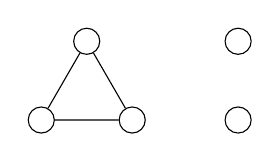
\begin{tikzpicture}
            \node (v1) at (0,0) [circle, draw] {};
            \node (v2) at (1.155,0) [circle, draw] {};
            \node (v3) at (0.577,1) [circle, draw] {};
            \draw (v1) -- (v2) -- (v3) -- (v1);

            \node (v4) at (2.5, 0) [circle, draw] {};
            \node (v5) at (2.5, 1) [circle, draw] {};
        \end{tikzpicture}
    \caption{\(C\) and two other vertices}
    \end{figure}

    Two subcases.

    First subcase.
    \begin{figure}[h!]
        \centering
        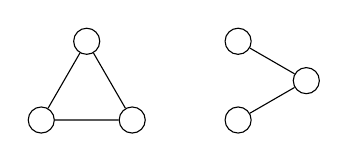
\begin{tikzpicture}
            \node (v1) at (0,0) [circle, draw] {};
            \node (v2) at (1.155,0) [circle, draw] {};
            \node (v3) at (0.577,1) [circle, draw] {};
            \draw (v1) -- (v2) -- (v3) -- (v1);

            \node (v4) at (2.5, 0) [circle, draw] {};
            \node (v5) at (2.5, 1) [circle, draw] {};
            \node (v6) at (3.366, 0.5) [circle, draw] {};
            \draw (v4) -- (v6) -- (v5);
        \end{tikzpicture}
    \end{figure}

    Second subcase.
    \begin{figure}[h!]
        \centering
        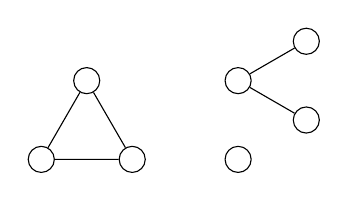
\begin{tikzpicture}
            \node (v1) at (0,0) [circle, draw] {};
            \node (v2) at (1.155,0) [circle, draw] {};
            \node (v3) at (0.577,1) [circle, draw] {};
            \draw (v1) -- (v2) -- (v3) -- (v1);

            \node (v4) at (2.5, 0) [circle, draw] {};
            \node (v5) at (2.5, 1) [circle, draw] {};
            \node (v6) at (3.366, 0.5) [circle, draw] {};
            \node (v7) at (3.366, 1.5) [circle, draw] {};
            \draw (v6) -- (v5) -- (v7);

        \end{tikzpicture}
    \end{figure}

    \textbf{Case 2:} \(C\) has length \(4\)

    \begin{figure}[h!]
        \centering
        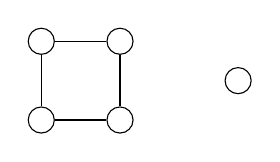
\begin{tikzpicture}
            \node (v1) at (0, 0) [circle, draw] {};
            \node (v2) at (1, 0) [circle, draw] {};
            \node (v3) at (1, 1) [circle, draw] {};
            \node (v4) at (0, 1) [circle, draw] {};
            \draw (v1) -- (v2) -- (v3) -- (v4) -- (v1);

            \node (v5) at (2.5, 0.5) [circle, draw] {};

        \end{tikzpicture}
    \end{figure}

    \textbf{Case 3:} \(C\) has length greater than \(5\) --
    Cleverly change which matching we choose and we can get a degree \(3\) vertex.

    \begin{figure}[h!]
        \centering
        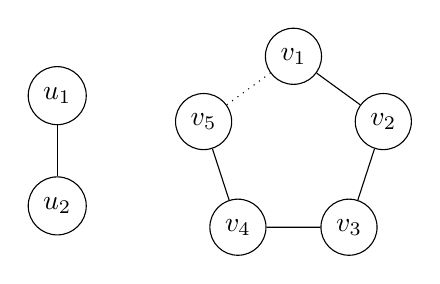
\begin{tikzpicture}
        \foreach \i in {1,...,5} \node (v\i) at ({162-72*\i}:1.2) [circle, draw] {\(v_{\i}\)};
        \draw (v1) -- (v2) -- (v3) -- (v4) -- (v5);

        \draw[dotted] (v5) -- (v1);

        \node (u1) at (-3,.7) [circle, draw] {\(u_1\)};
        \node (u2) at (-3,-.7) [circle, draw] {\(u_2\)};
        \draw (u1) -- (u2);
        \end{tikzpicture}
    \end{figure}

    \begin{figure}[h!]
        \centering
        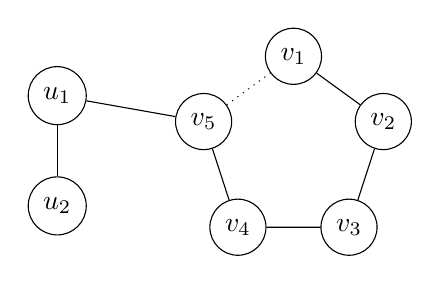
\begin{tikzpicture}
        \foreach \i in {1,...,5} \node (v\i) at ({162-72*\i}:1.2) [circle, draw] {\(v_{\i}\)};
        \draw (v1) -- (v2) -- (v3) -- (v4) -- (v5);

        \draw[dotted] (v5) -- (v1);

        \node (u1) at (-3,.7) [circle, draw] {\(u_1\)};
        \node (u2) at (-3,-.7) [circle, draw] {\(u_2\)};
        \draw (u1) -- (u2);

        \draw (u1) -- (v5);
        \end{tikzpicture}
    \end{figure}

\end{proof}

\begin{lem}
If \(n > m\) and \(C\) has length \(3\), then \(\Gamma - V(M) \cong K_3\) or \(\Gamma - V(M) \cong K_3 \cup K_1\).
\end{lem}

\begin{proof}
    Since \(\Gamma - V(M)\) cannot have more than \(4\) vertices and also contains \(C\),
    then either \(\Gamma - V(M)\) is just \(C\) or \(C\) and another isolated vertex.

    In the later case, this isolated vertex cannot be connected to \(C\) otherwise
    we would have a degree \(3\) vertex.
\end{proof}

\begin{lem}
If \(n > m\) and \(C\) has length \(4\), then \(\Gamma - V(M) \cong K_{2,2}\)
\end{lem}

\begin{proof}
Since \(\Gamma - V(M)\) contains \(C\) and has at most \(4\) vertices,
\(\Gamma - V(M)\) is just \(C\) which isomorphic to \(K_{2,2}\).
\end{proof}


Abrams already studied the case when \(n = m\) in detail but we analyze it here for completeness.
\begin{lem}
If \(n = m\), then \(\Gamma - V(M)\) has at most \(4\) vertices.
\end{lem}

\begin{proof}
    Suppose \(\Gamma - V(M)\) has more than \(4\) vertices.
    This argument is similar to the \(n > m\) case where we proceed by cases on the length of \(C\).

    \textbf{Case 1:} \(C\) has length \(3\).

    \textbf{Case 2:} \(C\) has length \(4\).

    \textbf{Case 3:} \(C\) has length greater than \(4\).

\end{proof}

\begin{lem}
If \(n = m\) and \(C\) has length \(3\), then \(\Gamma - V(M) \cong K_3\).
\end{lem}

\begin{lem}
If \(n = m\) and \(C\) has length \(4\), then \(\Gamma - V(M) \cong K_{2,2}\).
\end{lem}


